\documentclass[acmsmall,nonacm=true,screen=true]{acmart}
\settopmatter{printfolios=false,printccs=false,printacmref=false}

%%%%%%%%%%%%%%%%%%%%%%%%%%%%%%%%%%%%%%%%%%
%% Bibliography style
%%%%%%%%%%%%%%%%%%%%%%%%%%%%%%%%%%%%%%%%%%
\bibliographystyle{ACM-Reference-Format}
\citestyle{acmauthoryear}

%%%%%%%%%%%%%%%%%%%%%%%%%%%%%%%%%%%%%%%%%%
%% Packages
%%%%%%%%%%%%%%%%%%%%%%%%%%%%%%%%%%%%%%%%%%

% URLs
\newcommand\site[1]{\footnote{\url{#1}}}

% Quotes
\usepackage{csquotes}

% Graphics
\graphicspath{ {images/} }
\usepackage{colortbl}

% Tikz
\usepackage{tikz}
\usetikzlibrary{chains,arrows,automata,fit,positioning,calc}

% Import Agda code
\newcommand\nat{
\begin{code}%
\>[0]\AgdaKeyword{data}\AgdaSpace{}%
\AgdaDatatype{ℕ}\AgdaSpace{}%
\AgdaSymbol{:}\AgdaSpace{}%
\AgdaPrimitiveType{Set}\AgdaSpace{}%
\AgdaKeyword{where}\<%
\\
\>[0][@{}l@{\AgdaIndent{0}}]%
\>[2]\AgdaInductiveConstructor{zero}%
\>[8]\AgdaSymbol{:}\AgdaSpace{}%
\AgdaDatatype{ℕ}\<%
\\
%
\>[2]\AgdaInductiveConstructor{suc}%
\>[8]\AgdaSymbol{:}\AgdaSpace{}%
\AgdaDatatype{ℕ}\AgdaSpace{}%
\AgdaSymbol{→}\AgdaSpace{}%
\AgdaDatatype{ℕ}\<%
\\
%
\\[\AgdaEmptyExtraSkip]%
\>[0]\AgdaOperator{\AgdaFunction{\AgdaUnderscore{}+\AgdaUnderscore{}}}\AgdaSpace{}%
\AgdaSymbol{:}\AgdaSpace{}%
\AgdaDatatype{ℕ}\AgdaSpace{}%
\AgdaSymbol{→}\AgdaSpace{}%
\AgdaDatatype{ℕ}\AgdaSpace{}%
\AgdaSymbol{→}\AgdaSpace{}%
\AgdaDatatype{ℕ}\<%
\\
\>[0]\AgdaInductiveConstructor{zero}%
\>[7]\AgdaOperator{\AgdaFunction{+}}\AgdaSpace{}%
\AgdaBound{n}\AgdaSpace{}%
\AgdaSymbol{=}\AgdaSpace{}%
\AgdaBound{n}\<%
\\
\>[0]\AgdaInductiveConstructor{suc}\AgdaSpace{}%
\AgdaBound{m}%
\>[7]\AgdaOperator{\AgdaFunction{+}}\AgdaSpace{}%
\AgdaBound{n}\AgdaSpace{}%
\AgdaSymbol{=}\AgdaSpace{}%
\AgdaInductiveConstructor{suc}\AgdaSpace{}%
\AgdaSymbol{(}\AgdaBound{m}\AgdaSpace{}%
\AgdaOperator{\AgdaFunction{+}}\AgdaSpace{}%
\AgdaBound{n}\AgdaSymbol{)}\<%
\end{code}
}


%%%%%%%%%%%%%%%%%%%%%%%%%%%%%%%%%%%%%%%%%%
%% Macros
%%%%%%%%%%%%%%%%%%%%%%%%%%%%%%%%%%%%%%%%%%
\newcommand\todo[1]{\textcolor{red}{TODO: #1}}

\begin{document}

%%%%%%%%%%%%%%%%%%%%%%%%%%%%%%%%%%%%%%%%%%
%% Title
%%%%%%%%%%%%%%%%%%%%%%%%%%%%%%%%%%%%%%%%%%
\title{Formal investigation of the Extended UTxO model}
\subtitle{Laying the foundations for the formal verification of smart contracts}

%%%%%%%%%%%%%%%%%%%%%%%%%%%%%%%%%%%%%%%%%%
%% Authors
%%%%%%%%%%%%%%%%%%%%%%%%%%%%%%%%%%%%%%%%%%
\author{Orestis Melkonian}
\orcid{0000-0003-2182-2698}
\affiliation{
  \position{MSc Student}
  \department{Information and Computing Sciences}
  \institution{Utrecht University}
  \city{Utrecht}
  \country{The Netherlands}
}
\email{melkon.or@gmail.com}

%%%%%%%%%%%%%%%%%%%%%%%%%%%%%%%%%%%%%%%%%%
%% Abstract
%%%%%%%%%%%%%%%%%%%%%%%%%%%%%%%%%%%%%%%%%%
\begin{abstract}
This report serves as the proposal of my MSc thesis, supervised by Wouter Swierstra from
Utrecht University and Manuel Chakravarty from IOHK.
\end{abstract}

\maketitle

%%%%%%%%%%%%%%%%%%%%%%%%%%%%%%%%%%%%%%%%%%
\section{Introduction}
\label{sec:intro}
%%%%%%%%%%%%%%%%%%%%%%%%%%%%%%%%%%%%%%%%%%

% Distributed ledger technology creates issues
Although blockchain technology has opened a whole array of interesting new applications
(e.g. secure multi-party computation\cite{mpc}, fair protocol design fair\cite{fair}, zero-knowledge proof systems\cite{zeroproof}), 
reasoning about the behaviour of such systems is an exceptionally hard task. This is partly due to their concurrent nature, but
also the fiscal nature of the majority of the applications, which require a much higher degree of rigorousness compared to
conventional IT applications.

% Smart contracts create issues
The advent of smart contracts (programs that run on the blockchain itself) gave
rise to another source of vulnerabilities.
One primary example of such a vulnerability caused by the use of smart contracts is the
DAO attack\site{https://en.wikipedia.org/wiki/The_DAO_(organization)},
where a security flaw on the model of Ethereum's scripting language led to the exploitation of a venture capital fund
worth 150 million dollars at the time.
The solution was to create a hard fork of the Ethereum blockchain, clearly going against the decentralized spirit
of cryptocurrencies.
Since these (possibly Turing-complete) programs often deal with transactions of significant funds,
it is of utmost importance that one can reason and ideally provide formal proofs about their behaviour
in a concurrent/distributed setting.

% Aim of thesis
\paragraph{Research Question}
The aim of this thesis is to provide a mechanized formal model of an abstract distributed ledger equipped with
smart contracts, in which one can begin to formally investigate the expressiveness of the extended UTxo model.
Moreover, we hope to lay down firm grounds, onto which one can further conduct a formal comparison with account-based
models used in Ethereum. Put concisely, the research question posed is:
\begin{displayquote}
	\textit{How much expressiveness do we gain by extending the UTxO model?} \\
	\textit{Is it as expressive as the account-based model used in Ethereum?}
\end{displayquote}

\paragraph{Overview}
% Background
Section~\ref{sec:background} reviews some basic definitions related to blockchain
technology and introduces important literature, which will be the main subject of study
throughout the development of our reasoning framework.
% Methodology
Section~\ref{sec:methodology} describes the technology we will use to formally reason
about the problem at hand and some key design decisions we set upfront.
% Results
Section~\ref{sec:results} presents the progress made thus far in terms of (mechanized) formal verification,
as well as problems we have encountered and also expect along the way.
% Planning
Section~\ref{sec:plan} discusses next steps for the remainder of the thesis, as well as a rough estimate
on when these milestones will be completed.

%%%%%%%%%%%%%%%%%%%%%%%%%%%%%%%%%%%%%%%%%%
\section{Background}
\label{sec:background}
%%%%%%%%%%%%%%%%%%%%%%%%%%%%%%%%%%%%%%%%%%

% ?? Add cryptography section for:
%   1. hashes
%   2. private-pub key pairs for encryption/authentication

\subsection{Distributed Ledger Technology: Blockchain} \label{subsec:dlt}
Cryptocurrencies rely on distributed ledgers, where there is no central authority managing the accounts
and keeping track of the history of transactions.

One particular instance of distributed ledgers are blockchain systems, where (unrelated) transaction are
bundled together in blocks, which are linearly connected with hashes and distributed to all participants/peers.
The blockchain system, along with a consensus protocol deciding on which competing fork of the chain is to be included,
maintains an immutable distributed ledger (i.e. the history of transactions).

Validity of the transactions is tightly coupled with a consensus protocol, which makes sure
peers in the network only validate well-behaved/truthful transactions and are, moreover,
properly incentivized to do so.

The absence of a single central authority that has control over all assets of the participants allows
for shared control of the evolution of data (in this case transactions)
and generally leads to more robust and fair management of assets.

While cryptocurrencies are the major application of blockchain systems, one could easily
use them for any kind of valuable assets, or even as general distributed databases.

\subsection{Smart Contracts} \label{subsec:smartcontracts}
Most blockchain systems come equipped with a scripting language, where one can write
\textit{smart contracts} that dictate how a transaction operates. A smart contract
could, for instance, pose restrictions on who can redeem the output funds of a transaction.

One could view smart contracts as a replacement of legal frameworks, providing the means
to conduct contractual relationships completely algorithmically.

While previous work on writing financial contracts~\cite{spj} suggests it
is fairly straightforward to write such programs embedded in a general-purpose
language (in this case Haskell) and to reason about them with \textit{equational reasoning},
it is restricted in the centralized setting and, therefore, does not suffice for our needs.

Things become much more complicated when we move to the distributed/blockchain setting, as
can be evidenced by the current attempts being made to overcome this~\cite{setzer,short,scilla}.
Hence, there is a growing need for methods and tools that will
enable tractable and precise reasoning about such systems.

Numerous scripting languages have appeared recently~\cite{scriptlangs}, spanning a wide
spectrum of expressiveness and complexity. While language design can impose restrictions
on what can a language express, most of these restriction are inherited from
the accounting model that the underlying system adhere to.

In the next section, we will discuss the two main forms of accounting models:
\begin{enumerate}
\item \textbf{UTxO-based}: stateless models based on \textit{unspent transaction outputs}
\item \textbf{Account-based}: stateful models that explicitly model interaction between \textit{user accounts}
\end{enumerate}

\subsection{UTxO-based: Bitcoin} \label{subsec:bitcoin}
The primary example of a UTxO-based blockchain is Bitcoin~\cite{bitcoin}.
Its blockchain is a linear sequence of \textit{blocks} of transactions,
starting from the initial \textit{genesis} block.
Essentially, the blockchain acts as public log of all transactions that have taken place, where
each transaction refers to outputs of previous transactions,
except for the initial \textit{coinbase} transaction of each block.
Coinbase transactions have no inputs, create new currency and reward the miner of that block with a fixed amount.
Bitcoin also provides a cryptographic protocol to make sure no adversary can tamper with the transactional history,
e.g. by making the creation of new blocks computationally hard and invalidating the "truthful" chain statistically impossible.

A crucial aspect of Bitcoin's design is that there are no explicit addresses included in the transactions.
Rather, transaction outputs are actually program scripts, which allow someone to claim the funds by giving the proper inputs.
Thus, although there are no explicit user accounts in transactions, the effective available funds of a user
are all the \textit{unspent transaction outputs} (UTxO) that he can claim (e.g. by providing a digital signature).

\subsubsection{\textsc{Script}}
In order to state such scripts in the outputs of a transaction, Bitcoin provides a low-level, Forth-like,
stack-based scripting language, called \textsc{Script}.
\textsc{Script} is intentionally not Turing-complete (e.g. it does not provide looping structures),
in order to have more predictable behaviour.
Moreover, only a very restricted set of ``template" programs are considered standard, i.e.
allowed to be relayed from node to node.

\newcommand\ttt{\texttt}
\newcommand\stack[1]{\text{\ttt{#1}}}
\newcommand\Semantics[1]{\llbracket \stack{#1} \rrbracket}

\paragraph{P2PKH}
The most frequent example of a 'standard' program in \textsc{Script} is the
\textit{pay-to-pubkey-hash} (P2PKH) type of scripts. Given a hash of public key \texttt{<pub\#>},
a P2PKH output carries the following script:
\[
  \stack{OP\_DUP OP\_HASH <pub\#> OP\_EQ OP\_CHECKSIG}
\]
where \ttt{OP\_DUP} duplicates the top element of the stack, \ttt{OP\_HASH} replaces the top element with its hash,
\ttt{OP\_EQ} checks that the top two elements are equal, \ttt{OP\_CHECKSIG} verifies that the top two elements
are a valid pair of a digital signature of the transaction data and a public key hash.

The full script will be run when the output is claimed (i.e. used as input in a future transaction)
and consists of the P2PKH script, preceded by the digital signature of the transaction by its owner and a hash of
his public key. Given a digital signature \ttt{<sig>} and a public key hash \ttt{<pub>}, a transaction is valid
when the execution of the script below evaluates to \ttt{True}.
\[
  \stack{<sig> <pub> OP\_DUP OP\_HASH <pub\#> OP\_EQ OP\_CHECKSIG}
\]

To clarify, assume a scenario where Alice want to pay Bob \bitcoin ~10.
Bob provides Alice with the cryptographic hash of his public key (\ttt{<pub\#>})
and Alice can submit a transaction of \bitcoin ~10 with the following output script:
\[
  \stack{OP\_DUP OP\_HASH <pub\#> OP\_EQ OP\_CHECKSIG}
\]
After that, Bob can submit another transaction that uses this output by providing the digital signature
of the transaction \ttt{<sig>} (signed with his private key) and his public key \ttt{<pub>}.
It is easy to see that the resulting script evaluates to \ttt{True}.

\paragraph{P2SH}
A more complicated script type is \textit{pay-to-script-hash} (P2SH), where output scripts simply authenticate
against a hash of a \textit{redeemer} script \ttt{<red\#>}:
\[
  \stack{OP\_HASH <red\#> OP\_EQ}
\]

A redeemer script \ttt{<red>} resides in an input which uses the corresponding output. The following two conditions
must hold for the transaction to go through:
\begin{enumerate}
\item $\Semantics{<red>} = \stack{True}$
\item $\Semantics{<red> OP\_HASH <red\#> OP\_EQ} = \stack{True}$
\end{enumerate}
Therefore, in this case the script residing in the output are simpler, but inputs can also contain arbitrary redeemer scripts
(as long as they are of a standard ``template").

In this thesis, we will model scripts in a much more general, mathematical sense, so
we will eschew from any further investigation of properties particular to \textsc{Script}.

\subsubsection{The BitML Calculus}
Although Bitcoin is the most widely used blockchain to date, many aspects of it are poorly documented.
In general, there is a scarcity of formal models, most of which are either introductory or exploratory.

One of the most involved and mature previous work on formalizing the operation of Bitcoin
is the Bitcoin Modelling Language (BitML)~\cite{bitml}. First, an idealistic \textit{process calculus}
that models Bitcoin contracts is introduced, along with a detailed small-step reduction semantics that
models how contracts interact and its non-determinism accounts for the various outcomes.

The semantics consist of transitions between \textit{configurations}, abstracting away all the
cryptographic machinery and implementation details of Bitcoin.
Consequently, such operational semantics allow one to reason about the concurrent behaviour of
the contracts in a \textit{symbolic} setting.

The authors then provide a compiler from BitML contracts to 'standard' Bitcoin transactions, proven
correct via a correspondence between the symbolic model and the computational model operating on
the Bitcoin blockchain. We will return for a more formal treatment of BitML in Section~\ref{subsec:bitml}.

\subsubsection{Extended UTxO}
In this work, we will consider the version of the UTxO model used by IOHK's Cardano\site{www.cardano.org} blockchain.
In contrast to Bitcoin's \textit{proof-of-work} consensus protocol~\cite{bitcoin}, 
Cardano's \textit{Ouroboros} protocol~\cite{ouroboros} is \textit{proof-of-stake}.
This, however, does not concern our study of the abstract accounting model, thus we
refrain from formally modelling and comparing different consensus techniques.

The actual extension we care about is the inclusion of \textit{data scripts} in transaction
outputs, which essentially provide the validation script in the corresponding input with additional
information of an arbitrary type.

This extension of the UTxO model has already been
implemented\site{https://github.com/input-output-hk/plutus/tree/master/wallet-api/src/Ledger}, but
only informally documented\site{https://github.com/input-output-hk/plutus/blob/master/docs/extended-utxo/README.md}.
The reason to extend the UTxO model with data scripts is to bring more expressive power to UTxO-based blockchains,
hoping that it is on par with Ethereum's account-based scripting model (see Section~\ref{subsec:ethereum}).

However, there is no formal argument to support this claim, and it is the goal of this thesis
to provide the first formal investigation of the expressiveness introduced by this extension.

\subsection{Account-based: Ethereum} \label{subsec:ethereum}
On the other side of the spectrum, lies the second biggest cryptocurrency today, Ethereum~\cite{ethereum}.
In contrast to UTxO-based systems, Ethereum has a built-in notion of user addresses and operates on a
stateful accounting model. It goes even further to distinguish \textit{human accounts}
(controlled by a public-private key pair) from \textit{contract accounts} (controlled by some EVM code).

This added expressiveness is also reflected in the quasi-Turing-complete low-level stack-based bytecode language
in which contract code is written, namely the \textit{Ethereum Virtual Machine} (EVM).
EVM is mostly designed as a target, to which other high-level user-friendly languages will compile to.

\paragraph{Solidity}
The most widely adopted language that targets the EVM is \textit{Solidity},
whose high-level object-oriented design makes writing common contract use-cases (e.g. crowdfunding campaigns, auctions)
rather straightforward.

One of Solidity's most distinguishing features is the concept of a contract's \textit{gas}; a limit to the amount
of computational steps a contract can perform.
At the time of the creation of a transaction, its owner specifies a certain amount of gas the contract can consume and
pays a transaction fee proportional to it. In case of complete depletion, all global state changes are reverted.
This is a necessary ingredient for smart contract languages that provide
arbitrary looping behaviour, since non-termination of the validation phase is certainly undesirable.

If time permits, we will initially provide a formal justification of Solidity and proceed to
formally compare the extended UTxO model against it.
Since Solidity is a fully-fledged programming language with lots of features
(e.g. static typing, inheritance, libraries, user-defined types), it makes sense to 
restrict our formal study to a compact subset of Solidity that is easy to reason about.
This is the approach also taken in Featherweight Java~\cite{featherweightjava}; a subset
of Java that omits complex features such as reflection, in favour of easier behavioural reasoning
and a more formal investigation of its semantics.
In the same vein, we will try to introduce a lightweight version of Solidity, which we will refer to as
\textit{Featherweight Solidity}.

%%%%%%%%%%%%%%%%%%%%%%%%%%%%%%%%%%%%%%%%%%
\section{Methodology}
\label{sec:methodology}
%%%%%%%%%%%%%%%%%%%%%%%%%%%%%%%%%%%%%%%%%%

\subsection{Scope}
At this point, we have to stress the fact that we are not aiming for a formalization of a fully-fledged 
blockchain system with all its bells and whistles, but rather focus on the underlying accounting model.
Therefore, we will omit details concerning cryptographic operations and aspects of the actual implementation
of such a system. Instead, we will work on an abstract layer that postulates the well-behavedness of these
subcomponents, which will hopefully lend itself to more tractable reasoning and
give us a clear overview of the essence of the problem.

Restricting the scope of our attempt is also motivated from the fact that individual
components such as cryptographic protocols are orthogonal to the functionality we study here.
This lack of tight cohesion between the components of the system allows one to 
and thus can be safely factored out and formalized independently.

It is important to note that this is not always the case for every domain. A prominent example of
this are operating systems, which consist of intricately linked subcomponents (e.g. drivers, memory modules),
thus making impossible to trivially divide the overall proof into small independent ones.
In order to overcome this complexity burden, one has to invent novel ways of modular proof mechanization, as
exemplified by \textit{CertiKOS}~\cite{certikos}, a formally verified concurrent OS.

\subsection{Proof Mechanization}
Fortunately, the sub-components of the system we are examining are not no interdependent,
thus lending themselves to separate treatment.
Nonetheless, the complexity of the sub-system we care about is still high and requires rigorous investigation.
Therefore, we choose to conduct our formal study in a mechanized manner, i.e. using a proof assistant
along the way and formalizing all results in Type Theory.
Proof mechanization will allow us to discover edge cases and increase the confidence of the model under investigation.

\subsection{Agda}
As our proof development vehicle, we choose Agda~\cite{agda}, a dependently-typed total functional language
similar to Haskell~\cite{haskell}.

Agda embraces the \textit{Curry-Howard correspondence}, which states that types are isomorphic to statements in
(intuitionistic) logic and their programs correspond to the proofs of these statements~\cite{itt}.
Through its unicode-based \textit{mixfix} notational system, one can easily translate a mathematical formula
into a valid Agda type. Moreover, programs closely follow the structure of the corresponding proof, e.g. induction
in the proof manifests itself as recursion in the program.

While Agda is not ideal for large software development, its flexible notation
and elegant design is suitable for rapid prototyping of new ideas and exploratory purposes.
We estimate not to hit such a barrier of complexity,
since we will stay on a fairly abstract level which postulates cryptographic operations and other implementation details.

\paragraph{Limitation}
The main limitation of Agda lies in its lack of a proper proof automation system.
While there has been work on providing Agda with such capabilities~\cite{agdaauto},
it requires moving to a meta-programming mindset which would be an additional programming hindrance.

A reasonable alternative would be to use Coq~\cite{coq}, which provides a pragmatic
script-like language for programming \textit{tactics}, i.e. programs that work on proof contexts and can
generate new sub-goals.
This approach to proof mechanization has, however, been criticized for widening the gap between informal proofs
and programs written in a proof assistant.
This clearly goes against the aforementioned principle of \textit{proofs-as-programs}.

\subsection{The IOHK approach}
At this point, we would like to mention the specific approach taken by IOHK\site{https://iohk.io/}.
In contrast to numerous other companies currently creating cryptocurrencies, its main focus
is on provably correct protocols with a strong focus on peer-reviewing and robust implementations, rather
than fast delivery of results.
This is evidenced by the choice of programming languages (Agda/Coq/Haskell/Scala)
-- all functional programming languages with rich type systems --
and the use of \textit{property-based testing}~\cite{quickcheck} for the production code.

IOHK's distinct feature is that it advocates a more rigorous development pipeline;
ideas are initially worked on paper by pure academics,
which create fertile ground for starting formal verification in Agda/Coq for more confident results, 
which result in a prototype/reference implementation in Haskell,
which informs the production code-base (also written in Haskell) on the properties that should be tested.

Since this thesis is done in close collaboration with IOHK, it is situated on the second step of aforementioned pipeline;
while there has been work on writing out papers about the extended UTxO model, there are still no formally verified results.

\subsection{Functional Programming Principles}
One last important manifestation of the functional programming principles behind IOHK is the choice
of a UTxO-based cryptocurrency itself.

One the one hand, one can view a UTxO ledger as a dataflow diagram, whose nodes are the submitted transactions
and edges represent links between transaction inputs and outputs.
On the other hand, account-based ledgers rely on a global state and transaction have a much more complicated
specification.

The key point here is that UTxO-based transaction are just pure mathematical functions, which are much more
straightforward to model and reason about.
Coming back to the principles of functional programming, one could contrast this with the difference between
functional and imperative programs.
One can use \textit{equational reasoning} for functional programs, due to their \textit{referential transparency},
while this is not possible for imperative programs that contain side-effectful commands.

%%%%%%%%%%%%%%%%%%%%%%%%%%%%%%%%%%%%%%%%%%
\section{Preliminary Results}
\label{sec:results}
%%%%%%%%%%%%%%%%%%%%%%%%%%%%%%%%%%%%%%%%%%
This section gives an overview of the progress made so far in the on-going Agda formalization of the two main objects of study,
namely the Extended UTxO model and the BitML calculus.
For the sake of brevity, we refrain from showing the full Agda code along with the complete proofs, but rather
provide the most important datatypes and formalized results and explain crucial design choices we made along the way.
Furthermore, we will omit notational burden imposed by technicalities particular to Agda, such as \textit{universe polymorphism}
and \textit{proof irrelevance}.

\subsection{Formal Model I: Extended UTxO} \label{subsec:eutxo}
We now set out to model the accounting model of a UTxO-based ledger.
All code is publicly available on Github\site{https://github.com/omelkonian/formal-utxo}.
Let us start with some basic types:
\UTXObasicTypes{}
Addresses are represented as natural numbers, since we do not care about details arising from the encoding in an
actual implementation. Bitcoin values are again represented as natural numbers, but we provide a prefix notation
to emphasize that a number corresponds to a bitcoin amount.

There is also the notion of the \textit{state} of a ledger, which will be provided to transaction scripts and allow
them to have stateful behaviour for more complicated schemes (e.g. imposing time constraints).
\UTXOstate{}
The state components have not been finalized yet, but can easily be extended later when we actually investigate
examples with expressive scripts that make use of state information, such as the current length of the ledger (\textit{height}).

As mentioned previously, we will not dive into the verification of the cryptological components of the model,
hence we postulate an \textit{irreversible} hashing function which, given any value of any type,
gives back an address (i.e. a natural number) and is furthermore injective (i.e. it is statistically impossible for two different
values to have the same hash).
\UTXOhash{}

\subsubsection{Transactions}
In order to model transactions that are part of a distributed ledger, we need to first define
transaction \textit{inputs} and \textit{outputs}.
\UTXOinsOutRefs{}
\textit{Output references} consist of the address that this output's transaction hashes to, 
as well as the index in this transaction's list of outputs.
\textit{Transaction inputs} refer to some previous output in the ledger, but also contain two types of scripts.
The \textit{redeemer} provides evidence of authorization to spend the output.
The \textit{validator} then checks whether this is so, having access to the current state of the ledger, the bitcoin output
and data provided by the redeemer and the \textit{data script} (residing in outputs).
It is also noteworthy that we immediately model scripts by their \textit{denotational semantics},
omitting unnecessary details relating to concrete syntax, lexing and parsing.

Transaction outputs send a bitcoin amount to a particular address, which either corresponds to a public key hash of a
blockchain participant (P2PKH) or a hash of a next transaction's script (P2SH).
Here, we opt to embrace the \textit{inherently-typed} philosophy of Agda and model available addresses as module parameters.
That is, we package the following definitions in a module with such a parameter, as shown below:
\UTXOoutTx{}
\textit{Transaction outputs} consist of a bitcoin amount and the address (out of the available ones) this amount is sent to,
as well as the data script, which provides extra information to the aforementioned validator and allows for more expressive schemes.
Investigating exactly the extent of this expressiveness is one of the main goals of this thesis.

For a transaction to be submitted, one has to check that each input can actually spend the output it refers to.
At this point of interaction, one must combine all scripts, as shown below:
\UTXOrunValidation{}
Note that the intermediate types carried by the respective input and output must align, evidenced by the
equality proof that is required as an argument.

\subsubsection{Unspent transaction outputs}
With the basic modelling of a ledger and its transaction in place, it is fairly straightforward to 
inductively define the calculation of a ledger's unspent transaction outputs:
\UTXOutxo{}

\subsubsection{Validity of transactions}
In order to submit a transaction, one has to make sure it is valid with respect to the current ledger.
We model validity as a record indexed by the transaction to be submitted and the current ledger:
\UTXOvalid{}
The first four conditions make sure the transaction references and types are well-formed, namely that
inputs refer to actual transactions (\textit{validTxRefs}, \textit{validOutputIndices})
which are unspent so far (\textit{validOutputRefs}), but also that intermediate types used in interacting
inputs and outputs align (\textit{validDataScriptTypes}).

The last three validation condition are more interesting, as they ascertain the submitted transaction is valid,
namely that the bitcoin values sum up properly (\textit{preservesValues}), no output is spent twice (\textit{noDoubleSpending}),
validation succeeds for each input-output pair (\textit{allInputsValidate}) and outputs hash to the hash of their corresponding 
validator script (\textit{validateValidHashes}).

The definition of lookup functions is omitted, as they are uninteresting. The only important design choice is that,
instead of modelling lookups as partial functions (i.e. returning \inlineMaybe{}), they require a membership
proof as an argument moving the responsibility to the caller (as evidences by their usage in the validity conditions).

\subsubsection{Weakening Lemma}

but it would make sense to be able to add 
without losing the validity of the ledger constructed thus far.

In order to do, we need to first expose the basic datatypes from inside the module,
introducing their \textit{primed} version which takes the corresponding module parameter as an index:

\UTXOprimedTypes{}

We can now precisely define what it means to weaken an address space; one just adds more available
addresses without removing any of the pre-existing addresses:

\UTXOweaken{}
For simplicity's sake, we allow extension at the end of the address space instead of anywhere in
between\footnote{Technically, we require \inlinePrefix{} instead of the more flexible \inlineSubset{}.}.
Notice also that the only place where weakening takes place are transaction outputs, since all other
components do not depend on the available address space.

With the weakening properly defined, we can finally prove the \textit{weakening lemma} for the available address space:

\UTXOweakenLemma{}
The weakening lemma states that the validity of a transaction with respect to a ledger is preserved if
we choose to weaken the available address space, which we estimate to be useful when we later prove more 
intricate properties of the extended UTxO model.

\subsubsection{Example} \label{subsec:utxo-example}
To showcase how we can use our model to construct \textit{correct-by-construction} ledgers,
let us revisit the example ledger presented in the Chimeric Ledgers paper~\cite{chimeric}.

Any blockchain can be visually represented as a \textit{directed acyclic graph} (DAG), with transactions as nodes 
and input-output pairs as edges, as shown in Figure~\ref{fig:utxo-ledger}.
\begin{figure}
\newcommand\forge[1]{forge: \bitcoin ~#1}
\newcommand\fee[1]{fee:\hspace{7pt} \bitcoin ~#1}
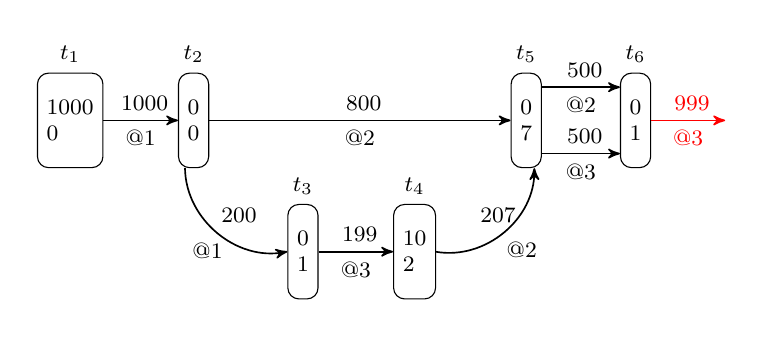
\begin{tikzpicture}
  [basic box/.style = {
     draw,
     shape = rectangle,
     align = left,
     %minimum width=2cm,
     minimum height=1.2cm,
     rounded corners},
   redge/.style = {
     bend right = 50},
   upedge/.style = {
     transform canvas={yshift=12pt}},
   downedge/.style = {
     transform canvas={yshift=-12pt}},
   to/.style = {
     ->,
     >=stealth',
     semithick},
  every matrix/.style={column sep=0.9cm},
  font=\footnotesize
  ]
  \matrix{
    \node[basic box, label = $t_1$] (t)
      {\forge{1000}\\ \fee{0}};
    & \node[basic box, label = $t_2$] (tt)
      {\forge{0}\\ \fee{0}};
    & \node {};
    & \node {};
    & \node[basic box, label = $t_5$] (tfive)
      {\forge{0}\\ \fee{7}};
    & \node[basic box, label = $t_6$] (tsix)
      {\forge{0}\\ \fee{1}};
    & \node (end) {}; \\
    
    \node {};
    & \node {};
    & \node[basic box, label = $t_3$] (ttt)
      {\forge{0}\\ \fee{1}};
    & \node[basic box, label = $t_4$] (tfour)
      {\forge{10}\\ \fee{2}};
    & \node {};
    & \node {};
    & \node {}; \\
  };

  \path
  (t)     edge[to]           node[anchor=south,above]{\bitcoin ~1000}
                             node[anchor=north,below]{@1} (tt)
  (tt)    edge[to, redge]    node[anchor=south,above]{\hspace{10pt} \bitcoin ~200}
                             node[anchor=north,below]{\hspace{-10pt} @1} (ttt)
  (tt)    edge[to]           node[anchor=south,above]{\bitcoin ~800}
                             node[anchor=north,below]{@2} (tfive)  
  (ttt)   edge[to]           node[anchor=south,above]{\bitcoin ~199}
                             node[anchor=north,below]{@3} (tfour)
  (tfour) edge[to, redge]    node[anchor=south,above]{\hspace{-10pt} \bitcoin ~207}
                             node[anchor=north,below]{\hspace{10pt} @2} (tfive)
  (tfive) edge[to, upedge]   node[anchor=south,above]{\bitcoin ~500}
                             node[anchor=north,below]{@2} (tsix)
  (tfive) edge[to, downedge] node[anchor=south,above]{\bitcoin ~500}
                             node[anchor=north,below]{@3} (tsix)
  (tsix)  edge[to, red]      node[anchor=south,above]{\bitcoin ~999}
                             node[anchor=north,below]{@3} (end)
  ;
\end{tikzpicture}
\caption{Example ledger with six transactions (unspent outputs are coloured in red)}
\label{fig:utxo-ledger}
\end{figure}

First, we need to set things up by declaring the list of available addresses and opening our module with this parameter.
\UTXOexampleSetup{}
Note that, since we will not utilize the expressive power of scripts in this example, we also provide convenient short cuts for
defining inputs and outputs with dummy default scripts.
Furthermore, we postulate that the addresses are actually the hashes of validators scripts, corresponding to the P2SH scheme
in Bitcoin.

We can then proceed to define the individual transactions depicted in Figure~\ref{fig:utxo-ledger}\footnote{
The first sub-index of each variable refers to the order the transaction are submitted,
while the second sub-index refers to which output of the given transaction we select.}:
\UTXOexampleA{}

Finally, we can construct a correct-by-construction ledger, by iteratively submitting each transaction along with
the proof that it is valid with respect to the ledger constructed thus far\footnote{
Here, we use a specialized notation of the form $\bullet t_1 \vdash p_1 \oplus t_2 \vdash p_2 \oplus \dots \oplus t_n \vdash p_n$,
where each insertion of transaction $t_x$ requires a proof of validity $p_x$ as well.
Technically, the $\oplus$ operator has type \inlineListCons{}.
}.
\UTXOexampleB{}
The proof validating the submission of the first transaction $t_1$ is trivially discharged.
While the rest of the proofs are quite involved, it is worthy to note that their size/complexity stays constant
independently of the ledger length. This is mainly due to the re-usability of proof components, arising from
the main functions being inductively defined.

It is now trivial to verify that the only unspent transaction output of our ledger is the output of the last
transaction $t_6$, as demonstrated below:
\UTXOexampleC{}

\subsection{Formal Model II: BitML Calculus} \label{subsec:bitml}
Now we move on to our second object of study, the BitML calculus for modelling smart contracts.

All code is publicly available on Github\site{https://github.com/omelkonian/formal-bitml}.
First, we begin with some basic definitions that will be used throughout this section:
\BITbasicTypes{}
Instead of giving a fixed datatype of participants, we parametrise our module with a given \textit{universe} of participants
and a non-empty list of honest participants.
Representation of time and monetary values is again done using natural numbers, while we model participant secrets as simple strings.
A deposits consists of the participant that owns it and the number of bitcoins it carries.
We, furthermore, introduce a simplistic language of logical predicates and arithmetic expressions with the usual constructs (e.g. numerical addition, logical conjunction) and give the usual semantics (predicates on booleans and arithmetic on naturals).
A more unusual feature of these expressions is the ability to calculate length of secrets (within arithmetic expressions)
and, in order to ensure more type safety later on, all expressions are indexed by the secrets they internally use.

\subsubsection{Contracts in BitML}
A \textit{contract advertisement} consists of a set of \textit{preconditions},
which require some resources from the involved participants prior to the contract's execution,
and a \textit{contract}, which specifies the rules according to which bitcoins are transferred between participants.

Preconditions either require participants to have a deposit of a certain value on their name (volatile or not) or 
commit to a certain secret. Notice the index of the datatype below, which captures all deposits required:
\BITpreconditions{}

Moving on to actual contracts, we define them by means of a collection of five types of commands;
\inlinePut{} injects participant deposits and revealed secrets in the remaining contract,
\inlineWithdraw{} transfers the current funds to a participant,
\inlineSplit{} distributes the current funds across different individual contracts,
\inlineAuthDecoration{} requires the authorization from a participant to proceed
and \inlineTimeDecoration{} allows further execution of the contract only after some time has passed.
\BITcontracts{}
There is a lot of type-level manipulation across all constructors, since we need to make sure that indices are
calculated properly. For instance, the total value in a contract constructed by the \inlineSplit{} command is the 
sum of the values carried by each branch.
The \inlinePut{} command\footnote{
\inlinePut{} comprises of several components and we will omit those that do not contain any helpful information,
e.g. write \inlineSimplePut{} when there are no revealed secrets and the predicate trivially holds.
} additionally requires an explicit proof that the predicate
of the \inlineIf{} part only uses secrets revealed by the same command.

We also introduce an intuitive syntax for declaring the different branches of a \inlineSplit{} command, emphasizing the
\textit{linear} nature of the contract's total monetary value:
\BITlollipop{}

Having defined both preconditions and contracts, we arrive at the definition of a contract advertisement:
\BITadvertisements{}
Notice that in order to construct an advertisement, one has to provide proof of the contract's validity with respect to
the given preconditions, namely that all deposit references in the contract are declared in the precondition
and each involved participant is required to have a persistent deposit.

To clarify things so far, let us see a simple example of a contract advertisement:
\\ \todo{Find a more intuitive example...}
\BITexampleAdvertisement{}
We first need to open our module with a fixed set of participants (in this case \inlineA{} and \inlineB{}).
We then define an advertisement, whose type already says a lot about what is going on;
it carries \bitcoin ~5, presumes the existence of at least one deposit of \bitcoin ~200, and requires the deposit
of \bitcoin ~200 and \bitcoin ~100 respectively.

Looking at the precondition itself, we see that the required deposits will be provided by \inlineB{} and \inlineA{}, respectively.
The contract first splits the bitcoins across three branches:
the first one gives \bitcoin ~2 to \inlineB{}, the second one gives \bitcoin ~2 to \inlineA{} after some time period,
while the third one retrieves \inlineB{}'s deposit of \bitcoin ~200 and allows \inlineB{} to authorise the
withdrawal of the remaining funds (currently \bitcoin ~201) from \inlineA{}.

We have omitted the proofs that ascertain the well-formedness of the \inlinePut{} and \inlineSplit{} commands, as
they are straightforward and do not provide any more intuition\footnote{
In fact, we have defined decidable procedures for all such proofs using the
\textit{proof-by-reflection} pattern~\cite{proofbyreflection}.
These automatically discharge all proof obligations, when there are no variables involved.}.

\subsubsection{Small-step Semantics}
BitML is a \textit{process calculus}, specialized for the case of smart contracts.
Contrary to most process calculi that provide primitive operators for inter-process communication via
message-passing~\cite{csp}, the BitML calculus does not provide such built-in features.

It, instead, provides domain-specific synchronization mechanisms through its \textit{small-step} reduction semantics.
These essentially define a \textit{labelled transition system} between \textit{configurations}, where
\textit{action} labels are emitted on every transition representing the required actions of the participants.
This symbolic model consists of two layers; the bottom one transitioning between \textit{untimed} configurations and the top one
that works on \textit{timed} configurations.

We start with the datatype of actions, which showcases the principal actions required to satisfy an advertisement's preconditions
and an action to pick one branch of a collection of contracts (introduced by the choice operator \inlineOplus{}).
We have omitted uninteresting actions concerning the manipulation of deposits, such as dividing, joining, donating and destroying them.
Since we will often need versions of the types of advertisements/contracts with their
indices existentially quantified, we first provide aliases for them.
\BITactions{}
The action datatype is parametrised\footnote{
In Agda, parameters are similar to indices, but are not allowed to vary across constructors.
}
over the participant who performs it
and includes several indices representing the prerequisites the current configuration has to satisfy, in order for
the action to be considered valid (e.g. one cannot spend a deposit to stipulate an advertisement that does not exist).

The first index refers to advertisements that appear in the current configuration, the second to contracts that have
already been stipulated, the third to deposits owned by the participant currently performing the action and the fourth
declares new deposits that will be created by the action
(e.g. dividing a deposit would require a single deposit as the third index and produce two other deposits in its fourth index).

Although are indexing scheme might seem a bit heavyweight now, it makes many little details and assumptions explicit,
which would bite us hard later on when we will need to reason about such entities.

Continuing from our previous example advertisement, let's see an example action where \inlineA{} spends the required \bitcoin ~100
to stipulate the example contract\footnote{
Notice that we have to make all indices of the advertisement explicit in the second index in the action's type signature.
}:
\BITactionExample{}

Configurations are now built from advertisements, active contracts, deposits, action authorizations and committed/revealed secrets:
\BITconfigurations{}
The indices are quite involved, since we need to record both the current advertisements, stipulated contracts and deposits
and the required ones for the configuration to become valid (i.e. closed). The most interesting case is the parallel composition
operator, where the resources provided by the left operand might satisfy some requirements of the right operand. Moreover,
consumed deposits have to be eliminated as there can be no double spending, while the number of advertisements and contracts
always grows.

By composing configurations together, we will eventually end up in a \textit{closed} configuration, where 
all required indices are empty (i.e. the configuration is self-contained):
\BITclosedConfigurations{}

We are now ready to declare the inference rules of the bottom layer of our small-step semantics,
by defining an inductive datatype modelling the binary step relation between untimed configurations:
\BITrules{}
There is a total of 18 rules we need to define, but we choose to depict only a representative subset of them.
The first pair of rules initially appends the authorisation to merge
two deposits to the current configuration (rule \inlineAuthJoinRule{}) and then performs the actual join (rule \inlineJoinRule{}).
This is a common pattern across all rules, where we first collect authorisations for an action by all involved participants,
and then we fire a subsequent rule to perform this action.
\inlineAdvertiseRule{} advertises a new contract, mandating that at least one of the participants involved in the pre-condition
is honest and requiring all deposits needed for stipulation are available in the surrounding context.
\inlineAuthCommitRule{} allows participants to commit to the secrets required by the contract's pre-condition, but only dishonest
ones can commit to the invalid length $\bot$.
Lastly, \inlineControlRule{} allows participants to give their authorization required by a particular branch out of the current
choices present in the contract, discarding any time constraints along the way.

It is noteworthy to mention that during the transcriptions of the complete set of rules from the paper~\cite{bitml}
to our dependently-typed setting,
we discovered a discrepancy in the \inlineAuthRevRule{} rule, namely that there was no context $\Gamma$.
Moreover, in order to later facilitate equational reasoning, we re-factored the \inlineControlRule{}
to not contain the inner step as a hypothesis, but instead immediately inject it in the result operand of the step relation.

A scrupulous reader might have noticed that the inference rules above have elided any treatment of timely constraints.
This is handled by the top layer, whose states are now timed configurations.
The only interesting inference rule is the one that handles time decorations of the form \inlineAfter{},
since all other cases are dispatched to the bottom layer (which just ignores timely aspects).
\BITtimedRules{}

Having defined the step relation in this way allows for equational reasoning, a powerful tool for
writing complex proofs:
\BITeqReasoning{}

\subsubsection{Example}
We are finally ready to see a more intuitive example of the \textit{timed-commitment protocol}, where a participant
commits to revealing a valid secret $a$ (e.g. "qwerty") to another participant,
but loses her deposit of \bitcoin ~1 if she does not meet a certain deadline $t$:
\BITexampleA{}

Below is one possible reduction in the bottom layer of our small-step semantics, demonstrating the case where
the participant actually meets the deadline:
\BITexampleB{}
At first, \inlineA{} holds a deposit of \bitcoin ~1, as required by the contract's precondition.
Then, the contract is advertised and the participants slowly provide the corresponding prerequisites
(i.e. \inlineA{} commits to a secret via \inlineAuthCommitRule{} and spends the required deposit via \inlineAuthInitRule{},
while \inlineB{} does not do anything).
After all pre-conditions have been satisfied, the contract is stipulated (rule \inlineInitRule{}) and the secret is successfully
revealed (rule \inlineAuthRevRule{}).
Finally, the first branch is picked (rule \inlineControlRule{}) and \inlineA{} retrieves her deposit back
(rules \inlinePutRevRule{} and \inlineWithdrawRule{}).

\subsection{Reasoning modulo permutation}
In the definitions above, we have assumed that \inlineMonoid{} forms a commutative monoid, which allowed us
to always present the required sub-configuration individually on the far left of a composite configuration.
While such definitions enjoy a striking similarity to the ones appearing in the original paper~\cite{bitml}
(and should always be preferred in an informal textual setting),
this approach does not suffice for a mechanized account of the model.
After all, this explicit treatment of all intuitive assumptions/details is what makes our approach robust and will lead to
a deeper understanding of how such these systems behave. 
To overcome this intricacy, we introduce an \textit{equivalence relation} on configurations, which holds when
they are just permutations of one another:
\BITreordering{}
Given this reordering mechanism, we now need to generalise all our inference rules to implicitly
reorder the current and next configuration of the step relation.
We achieve this by introducing a new variable for each of the operands of the resulting step relations,
replacing the operands with these variables and requiring that they are
re-orderings of the previous configurations, as shown in the following generalisation of the \inlineAuthJoinRule{} rule\footnote{
In fact, it is not necessary to reorder both ends for the step relation; at least one would be adequate.
}:
\BITgeneralRule{}

Unfortunately, we now have more proof obligations of the re-ordering relation lying around, which makes reasoning about
our semantics rather tedious. We are currently investigating different techniques to model such reasoning up to equivalence:
\begin{itemize}
\item \textit{Quotient types}~\cite{quotient} allow equipping a type with an equivalence relation.
If we assume the axiom that two elements of the underlying type are \textit{propositionally} equal when they are equivalent,
we could discharge our current proof burden trivially by reflexivity.
Unfortunately, while one can easily define \textit{setoids} in Agda, there is not enough support from the underlying type system to make reasoning about such an equivalence as easy as with built-in equality.
\item Going a step further into more advanced notions of equality, we arrive at \textit{homotopy type theory}~\cite{homotopy},
which tries to bridge the gap between reasoning about isomorphic objects in informal pen-paper proofs
and the way we achieve this in mechanized formal methods.
Again, realizing practical systems with such an enriched theory is a topic of current research~\cite{cubical} and no mature implementation exists yet, so we cannot integrate it with our current development in any pragmatic way.
\item The crucial problems we have encountered so far are attributed to the non-deterministic nature of BitML, which is actually
inherent in any process calculus. Building upon this idea, we plan to take a step back and investigate different reasoning
techniques for a minimal process calculus. Once we have an approach that is elegant and pragmatic, we will incorporate it
in our full-blown BitML calculus.
\end{itemize}

%%%%%%%%%%%%%%%%%%%%%%%%%%%%%%%%%%%%%%%%%%
\section{Planning}
\label{sec:plan}
%%%%%%%%%%%%%%%%%%%%%%%%%%%%%%%%%%%%%%%%%%
In this section, I describe possible next steps I plan to investigate during the remainder of my thesis.
It is impossible to accurately predict what will be achieved in the following five months
and there will definitely be some surprises along the way,
but I hope it will give realistic expectations of the final results of my thesis.

\subsection{Extended UTxO: Multi-currency}
Many major blockchain systems today support the creation of secondary cryptocurrencies, independent of the main  currency.
In Bitcoin, for instance, \textit{colored coins} allow transactions to assign additional meaning to their outputs
(e.g. each coin corresponding to a real-world asset, such as company shares)~\cite{coloredcoins}.

This approach, however, has the disadvantage of larger transactions and less efficient processing.
One could instead bake the multi-currency feature into the base system, mitigating the need for
larger transactions and slow processing.
Building on the abstract UTxO model, there are current research efforts on a general framework that provides mechanisms
to establish and enforce monetary policies for multiple currencies~\cite{multicurrency}.

Fortunately, the extensions proposed by the multi-currency are orthogonal to the functionality I have currently formalized.
In order to achieve this, one has to generalize the \inlineValue{} datatype to account for multiple currencies.
Hence, I plan to integrate this with my current formal development of the extended UTxO model and,
by doing so, provide the first formalization of a UTxO ledger that supports multiple cryptocurrencies.

\subsection{BitML Calculus}
Continuing my work on the formalization of the BitML paper~\cite{bitml},
there is still a lot of theoretical results to be covered:
\begin{itemize}
\item While I currently have the symbolic model in place, there is still no formalization of \textit{symbolic strategies},
where one can reason about different adversary strategies and prove that certain scenarios are impossible.
\item Another import task is to model the computational model; a counterpart of the symbolic model augmented
with pragmatic computational properties to more closely resemble the low-level details of Bitcoin.
\item When both symbolic and computational strategies have been formalized, I will be able to finally
prove the correctness of the BitML compiler, which translates high-level BitML contracts to
low-level standard Bitcoin transactions. The symbolic model concerns the input of the compiler, while
the computational one concerns the output.
This endeavour will involve implementing the actual translation and proving \textit{coherence} between the
symbolic and the computational model.
Proving coherence essentially requires providing a (weak) \textit{simulation} between the two models;
each step in the symbolic part is matched by (multiple) steps in the computational one.
\end{itemize}

\subsection{UTxO-BitML Integration}
So far I have worked separately on the two models under study, but it would be interesting to see whether these two
models can be intertwined in some way.
This would possibly involve a translation from BitML contracts to contracts modelled in our extended UTxO models,
along with corresponding meta-theoretical properties (e.g. validity of UTxO transactions correspond to another notion
of validity of BitML contracts).

Moreover, and it would be beneficial to review the different modelling techniques used across both models,
identifying their key strengths and witnesses.
With this in mind, I could refactor crucial parts of these two models for the sake of elegance, clarity and ease of reasoning.

\subsection{Plutus Integration}
In my current formalization of the extended UTxO model, scripts are immediately modelled by their denotations
(i.e. pure mathematical functions). This is not accurate, however, since scripts are actually pieces of program text.
However, there is current development by James Chapman of IOHK to formalize the meta-theory of Plutus,
Cardano's scripting language\site{https://github.com/input-output-hk/plutus-metatheory}.

Since we mostly care about Plutus as a scripting language, it would be possible to replace the denotations with
actual Plutus Core source code and utilize the formalized meta-theory to acquire the denotational semantics when needed.

\subsection{Featherweight Solidity}
One of the posed research questions concerns the expressiveness of the extended UTxO model with respect to
Ethereum-like account-based ledgers.

In order to investigate this in a formal manner, one has to initially model a reasonable subset of Solidity,
so a next step would be to model \textit{Featherweight Solidity}, taking inspiration from the
approach taken in the formalization of Java using \textit{Featherweight Java}~\cite{featherweightjava}.
Fortunately, I will not have to start from scratch, since there have been recent endeavours in F$^*$ to analyse and
verify Ethereum smart contracts, which already describe a simplified model of Solidity~\cite{short}.

As a next step, one could try out different example contracts in Solidity and check whether they can be transcribed to
contracts appropriate for an extended UTxO ledger.

\subsection{Proof Automation}
Last but not least, our current dependently-typed approach to formalizing our models has led to a significant proof burden,
as evidenced by the complicated type signatures presented throughout this proposal.
This certainly makes the reasoning process quite tedious and time consuming, so a reasonable task would be
to implement automatic proof-search procedures using Agda meta-programming~\cite{agdaauto}.

\subsection{Timetable}
I have assembled a detailed timetable in Figure~\ref{fig:workplan},
positioning the aforementioned tasks across the whole timespan of my thesis.

I expect to complete the tasks that are more tightly coupled with my current development, i.e.
incorporating multi-currency features and the formalized Plutus meta-theory into the extended UTxO model,
completing the formalization of the BitML paper and implementing proof-search automation to facilitate easier reasoning.
The merging of these two objects of study (i.e. UTxO and BitML) is somewhat unclear at this stage, but I hope
to at least provide a proof-of-concept translation, even if this comes without significant meta-theoretic results like coherence.

Other tasks, such as a mature model of Featherweight Solidity and formal results comparing it to UTxO,
are sadly outside the scope of this thesis due to time constraints.
Nonetheless, I will strive for a prototype model and implementation with lots of examples
and hope my work will lay the foundations to further investigate these topics in future research.

\begin{figure*}
  \centering
  \newcommand{\months}[1]{\multicolumn{#1}{c}{\cellcolor{hsblue2}} \\}
  \begin{tabular}{lcccccccc}
    \hline
    & 2018 & \multicolumn{7}{c}{2019} \\
    \hline
    & Dec & Jan & Feb & Mar & Apr & May & Jun & Jul \\
    \hline

    \textbf{UTxO} \\
    Basic abstract model                &      \months{2}
    Weakening lemma                     &&     \months{1}
    Extend with data scripts            &&&    \months{1}
    Multi-currency                      &&&&   \months{1}

    \textbf{BitML} \\
    Small-step Semantics                &      \months{3}
    Symbolic Model                      &&&&   \months{1}
    Computational Model                 &&&&   \months{1}
    Coherence                           &&&&&  \months{2}

    \textbf{UTxO-BitML Integration} \\
    Compiling BitML to UTxO             &&&&&  \months{2}
    
    \textbf{Plutus Integration} \\
    Model scripts with Plutus-Core      &&&&&& \months{1}
    
    \textbf{Evaluation} \\
    Featherweight Model                 &&&&&  \months{1}
    Example contracts                   &&&&&  \months{3}
    
    \textbf{Writeup} \\
    Write final thesis                  &&&&&& \months{3}
    
  \end{tabular}
  \caption{My workplan.}
  \label{fig:workplan}
\end{figure*}

%%%%%%%%%%%%%%%%%%%%%%%%%%%%%%%%%%%%%%%%%%
%% Bibliography
%%%%%%%%%%%%%%%%%%%%%%%%%%%%%%%%%%%%%%%%%%
\nocite{*} % T0D0 remove
\bibliography{sources}

\end{document}
